\def\mytitle{IDE ASSIGMNMENT}
\def\myauthor{PADIDAPU BHARGAV RAM}
\def\contact{padidapubhargavaram33@gmail.com}
\def\mymodule{Future Wireless Communications (FWC)}
\documentclass[journal,12pt,twocolumn]{IEEEtran}

\usepackage{setspace}
\usepackage{gensymb}
\usepackage{xcolor}
\usepackage{caption}
\usepackage[hyphens,spaces,obeyspaces]{url}
\usepackage[cmex10]{amsmath}
\usepackage{mathtools}
\singlespacing
\usepackage{amsthm}
\usepackage{mathrsfs}
\usepackage{txfonts}
\usepackage{stfloats}
\usepackage{cite}
\usepackage{cases}
\usepackage{subfig}
\usepackage{longtable}
\usepackage{multirow}
\twocolumn


\usepackage{graphicx}
\graphicspath{{./images/}}
\usepackage[colorlinks,linkcolor={black},citecolor={blue!80!black},urlcolor={blue!80!black}]{hyperref}
\usepackage[parfill]{parskip}
\usepackage{lmodern}
\usepackage{tikz}
\usepackage{circuitikz}
\usepackage{karnaugh-map}
\usepackage{pgf}
\usepackage[hyphenbreaks]{breakurl}

\usepackage{tabularx}
\usetikzlibrary{calc}

\renewcommand*\familydefault{\sfdefault}
\usepackage{watermark}
\usepackage{lipsum}
\usepackage{xcolor}
\usepackage{listings}
\usepackage{float}
\usepackage{titlesec}
\usepackage{enumitem}
\DeclareMathOperator*{\Res}{Res}
\renewcommand\thesection{\arabic{section}}
\renewcommand\thesubsection{\thesection.\arabic{subsection}}
\renewcommand\thesubsubsection{\thesubsection.\arabic{subsubsection}}

\renewcommand\thesectiondis{\arabic{section}}
\renewcommand\thesubsectiondis{\thesectiondis.\arabic{subsection}}
\renewcommand\thesubsubsectiondis{\thesubsectiondis.\arabic{subsubsection}}
\titlespacing{\subsection}{1pt}{\parskip}{3pt}
\titlespacing{\subsubsection}{0pt}{\parskip}{-\parskip}
\titlespacing{\paragraph}{0pt}{\parskip}{\parskip}
\newcommand{\figuremacro}[5]{
    \begin{figure}[#1]
        \centering
        \includegraphics[width=#5\columnwidth]{#2}
        \caption[#3]{\textbf{#3}#4}
        \label{fig:#2}
    \end{figure}
}

\lstset{
frame=single, 
breaklines=true,
columns=fullflexible
}
\title{\mytitle}
\author{\myauthor\hspace{1em}\\\contact\\IITH\hspace{0.5em}-\hspace{0.6em}\mymodule}
\date{20-12-2022}
\def\inputGnumericTable{}                                 %%
\lstset{
frame=single, 
breaklines =true,
columns= fullflexible
}
 \begin{document}
\theoremstyle{definition}
\newtheorem{theorem}{Theorem}[section]
\newtheorem{problem}{Problem}
\newtheorem{proposition}{Proposition}[section]
\newtheorem{lemma}{Lemma}[section]
\newtheorem{corollary}[theorem]{Corollary}
\newtheorem{example}{Example}[section]
\newtheorem{definition}{Definition}[section]
%\newtheorem{algorithm}{Algorithm}[section]
%\newtheorem{cor}{Corollary}
\newcommand{\BEQA}{\begin{eqnarray}}
\newcommand{\EEQA}{\end{eqnarray}}
\newcommand{\define}{\stackrel{\triangle}{=}}
%\bibliographystyle{IEEEtran}

\vspace{3cm}
\maketitle
\tableofcontents
  \section{\textbf{Question}}
  \begin{enumerate}     
\item The representation of the decimal number $(27.625)_{10}$ in base-2 number is
\begin{enumerate}[label=(\Alph*)]
    \item 11011.110
    \item 11101.101
    \item 11011.101
    \item 10111.110
\end{enumerate}
\end{enumerate}
\section{\textbf{Components}}
\begin{tabularx}{0.46\textwidth} { 
  | >{\centering\arraybackslash}X 
  | >{\centering\arraybackslash}X 
  | >{\centering\arraybackslash}X
  | >{\centering\arraybackslash}X | }
\hline
\textbf{Component}& \textbf{Values} & \textbf{Quantity}\\
\hline
Arduino & UNO & 1 \\  
\hline
JumperWires & M-F & 15 \\ 
\hline
LCD & &1\\
\hline
Bread board & & 1\\
\hline
     \end{tabularx}
\section{\textbf{LCD PINS}}
 \begin{figure}[H]
\centering
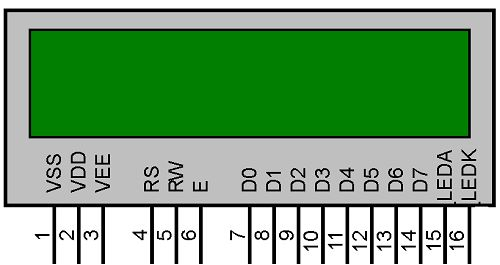
\includegraphics[width=\columnwidth]{figs/LCD.jpg}
\caption{LCD}
\label{fig:lcd}
\end{figure} 
\section{\textbf{Implementation}}
  \begin{tabularx}{0.46\textwidth} { 
  | >{\centering\arraybackslash}X 
  | >{\centering\arraybackslash}X  | }
\hline
\textbf{Arduino PIN} & \textbf{LCD} \\ 
\hline
D7 & RS\\
\hline
D8 & EN\\
\hline
D9 & 11\\
\hline
D10 & 12\\
\hline
D11 & 13\\
\hline
D12 & 14\\
\hline
5V & VCC\\
\hline
\end{tabularx}
\begin{center}
    Connections
\end{center}
\section{\textbf{Procedure}}
    1. Connect the circuit as per the above table.\\
    2. connect the LCD to Arduino UNO\\
\\ \begin{tabularx}{0.46\textwidth} { 
  | >{\centering\arraybackslash}X |}
  \hline
  https://github.com/Padidapu-Bhargav/Digital-Design/blob/main/Platformio-assignment.ino \\
  \hline
\end{tabularx}
    \section{\textbf{LCD OUTPUT}}
 \begin{figure}[H]
\centering
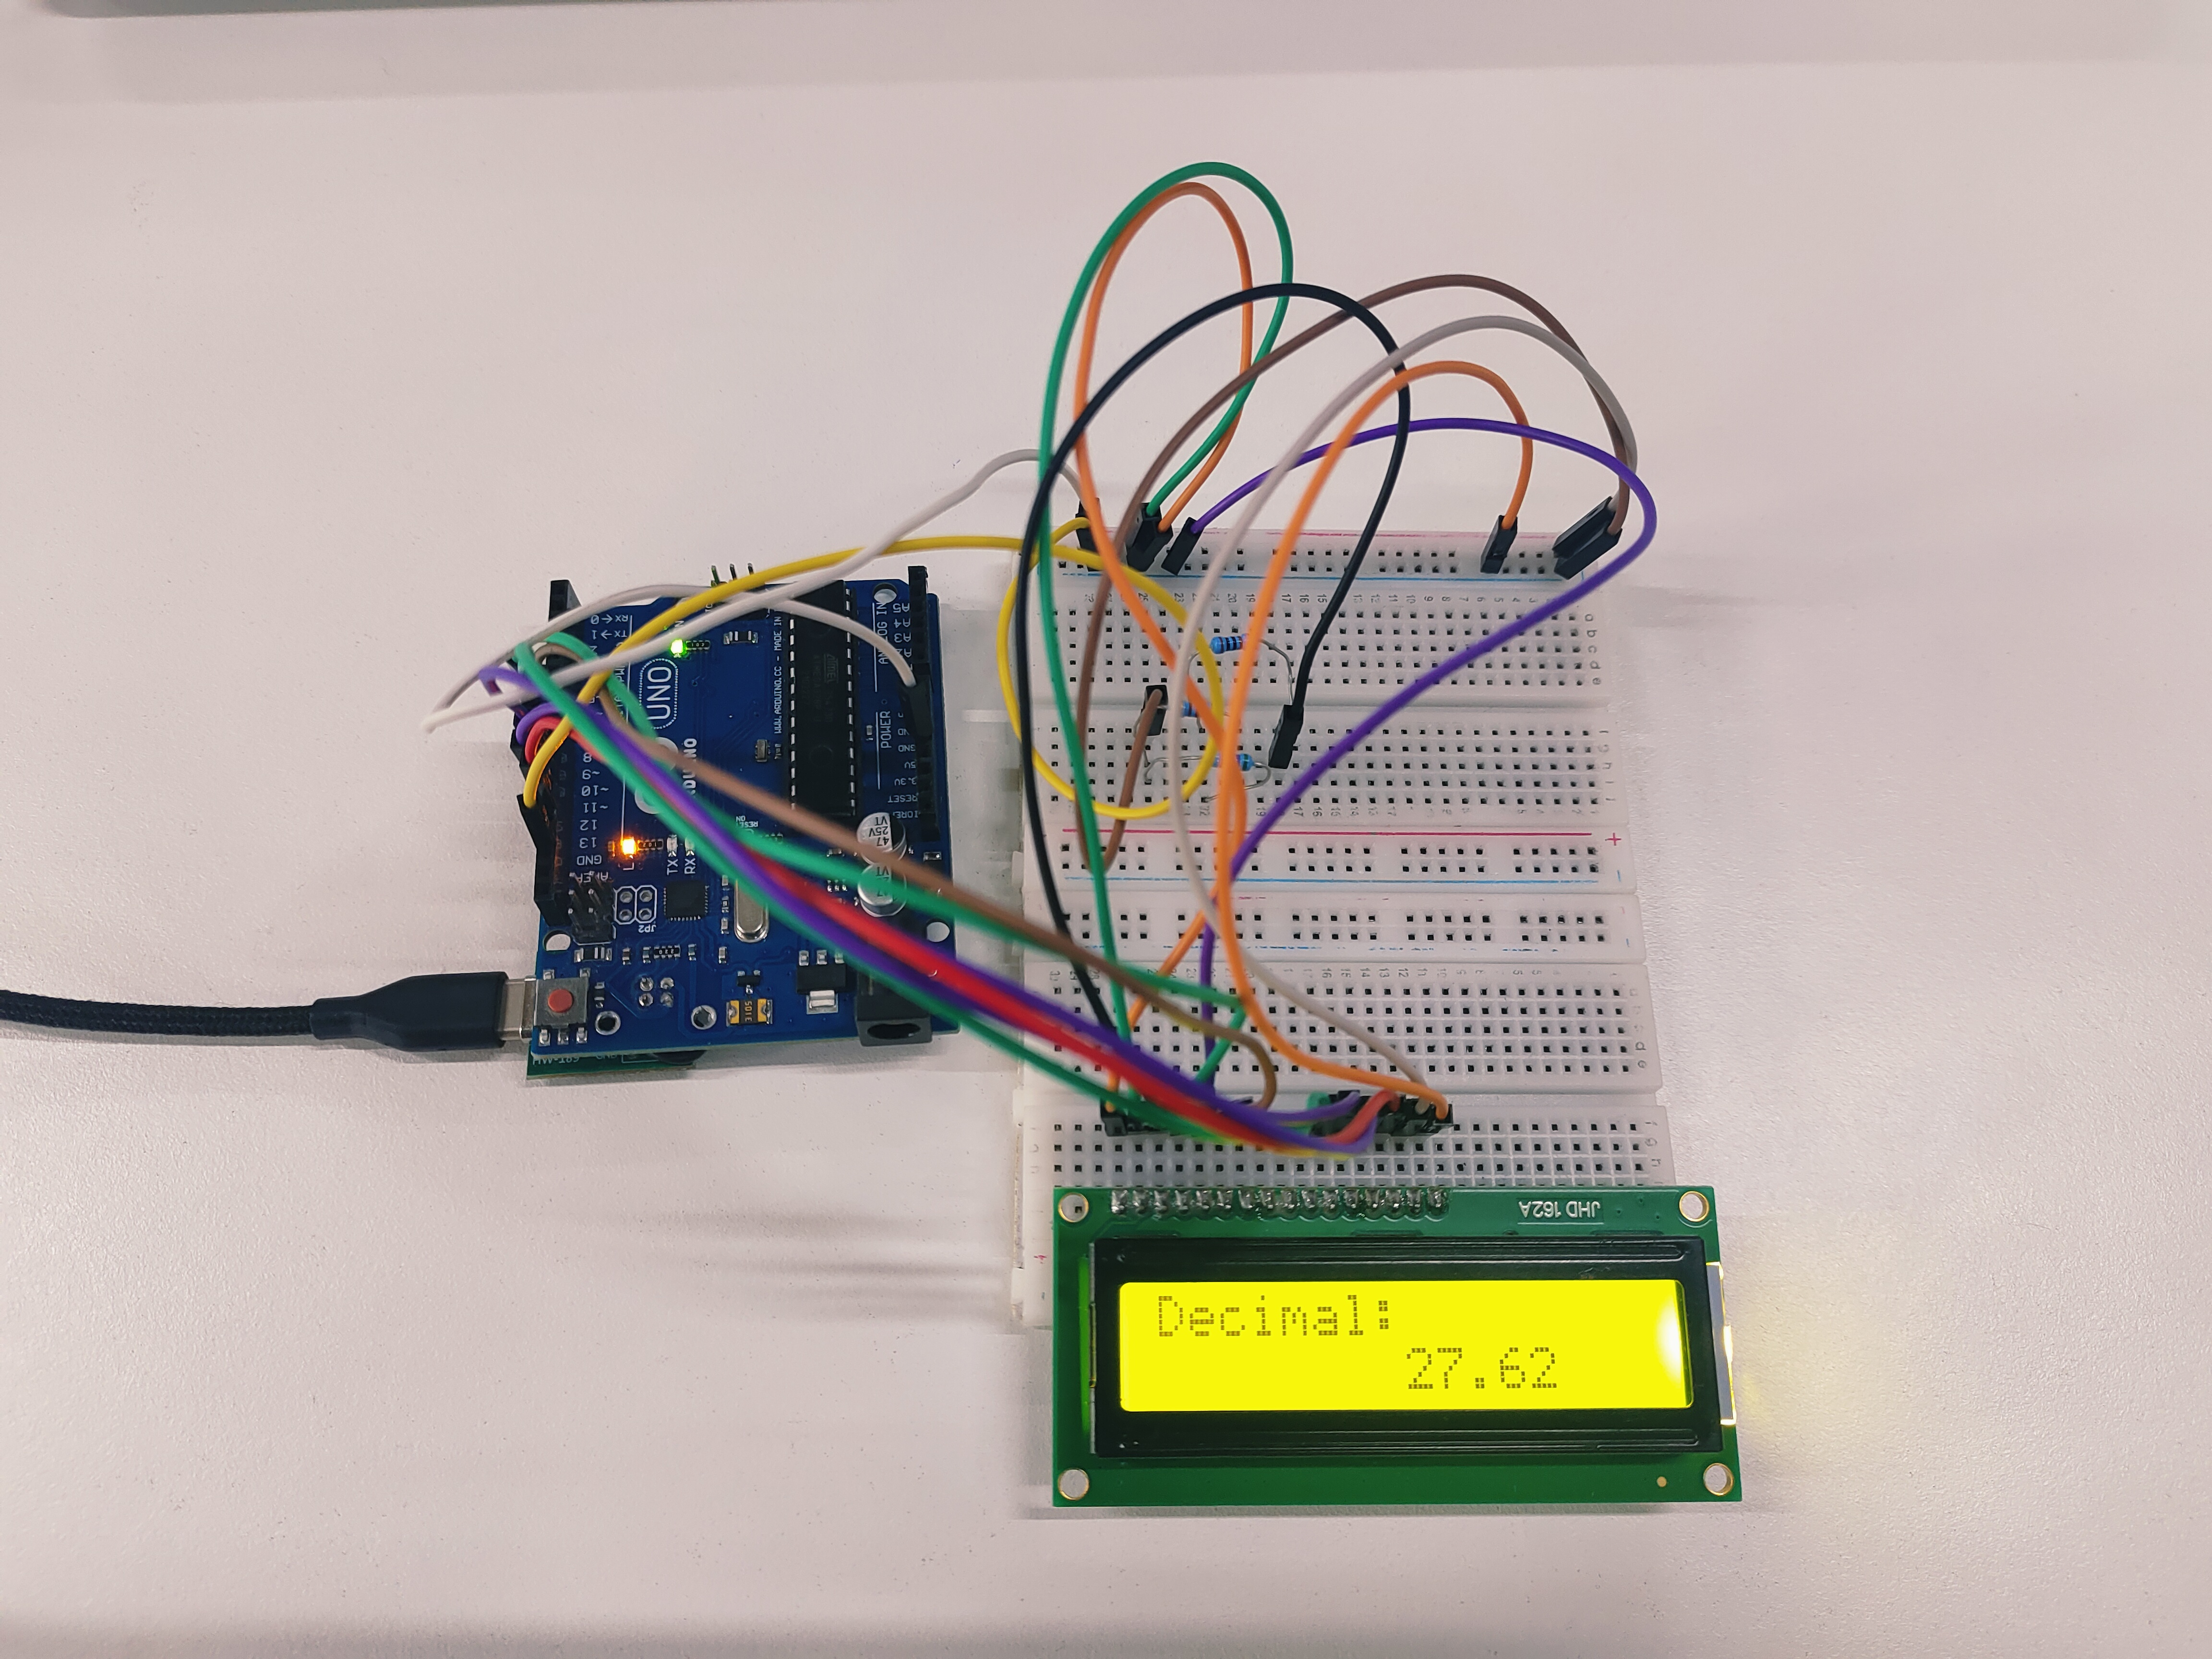
\includegraphics[width=\columnwidth]{figs/decimal_out.jpg}
\caption{Decimal value}
\label{fig:lcd}
\end{figure}

\begin{figure}[H]
\centering
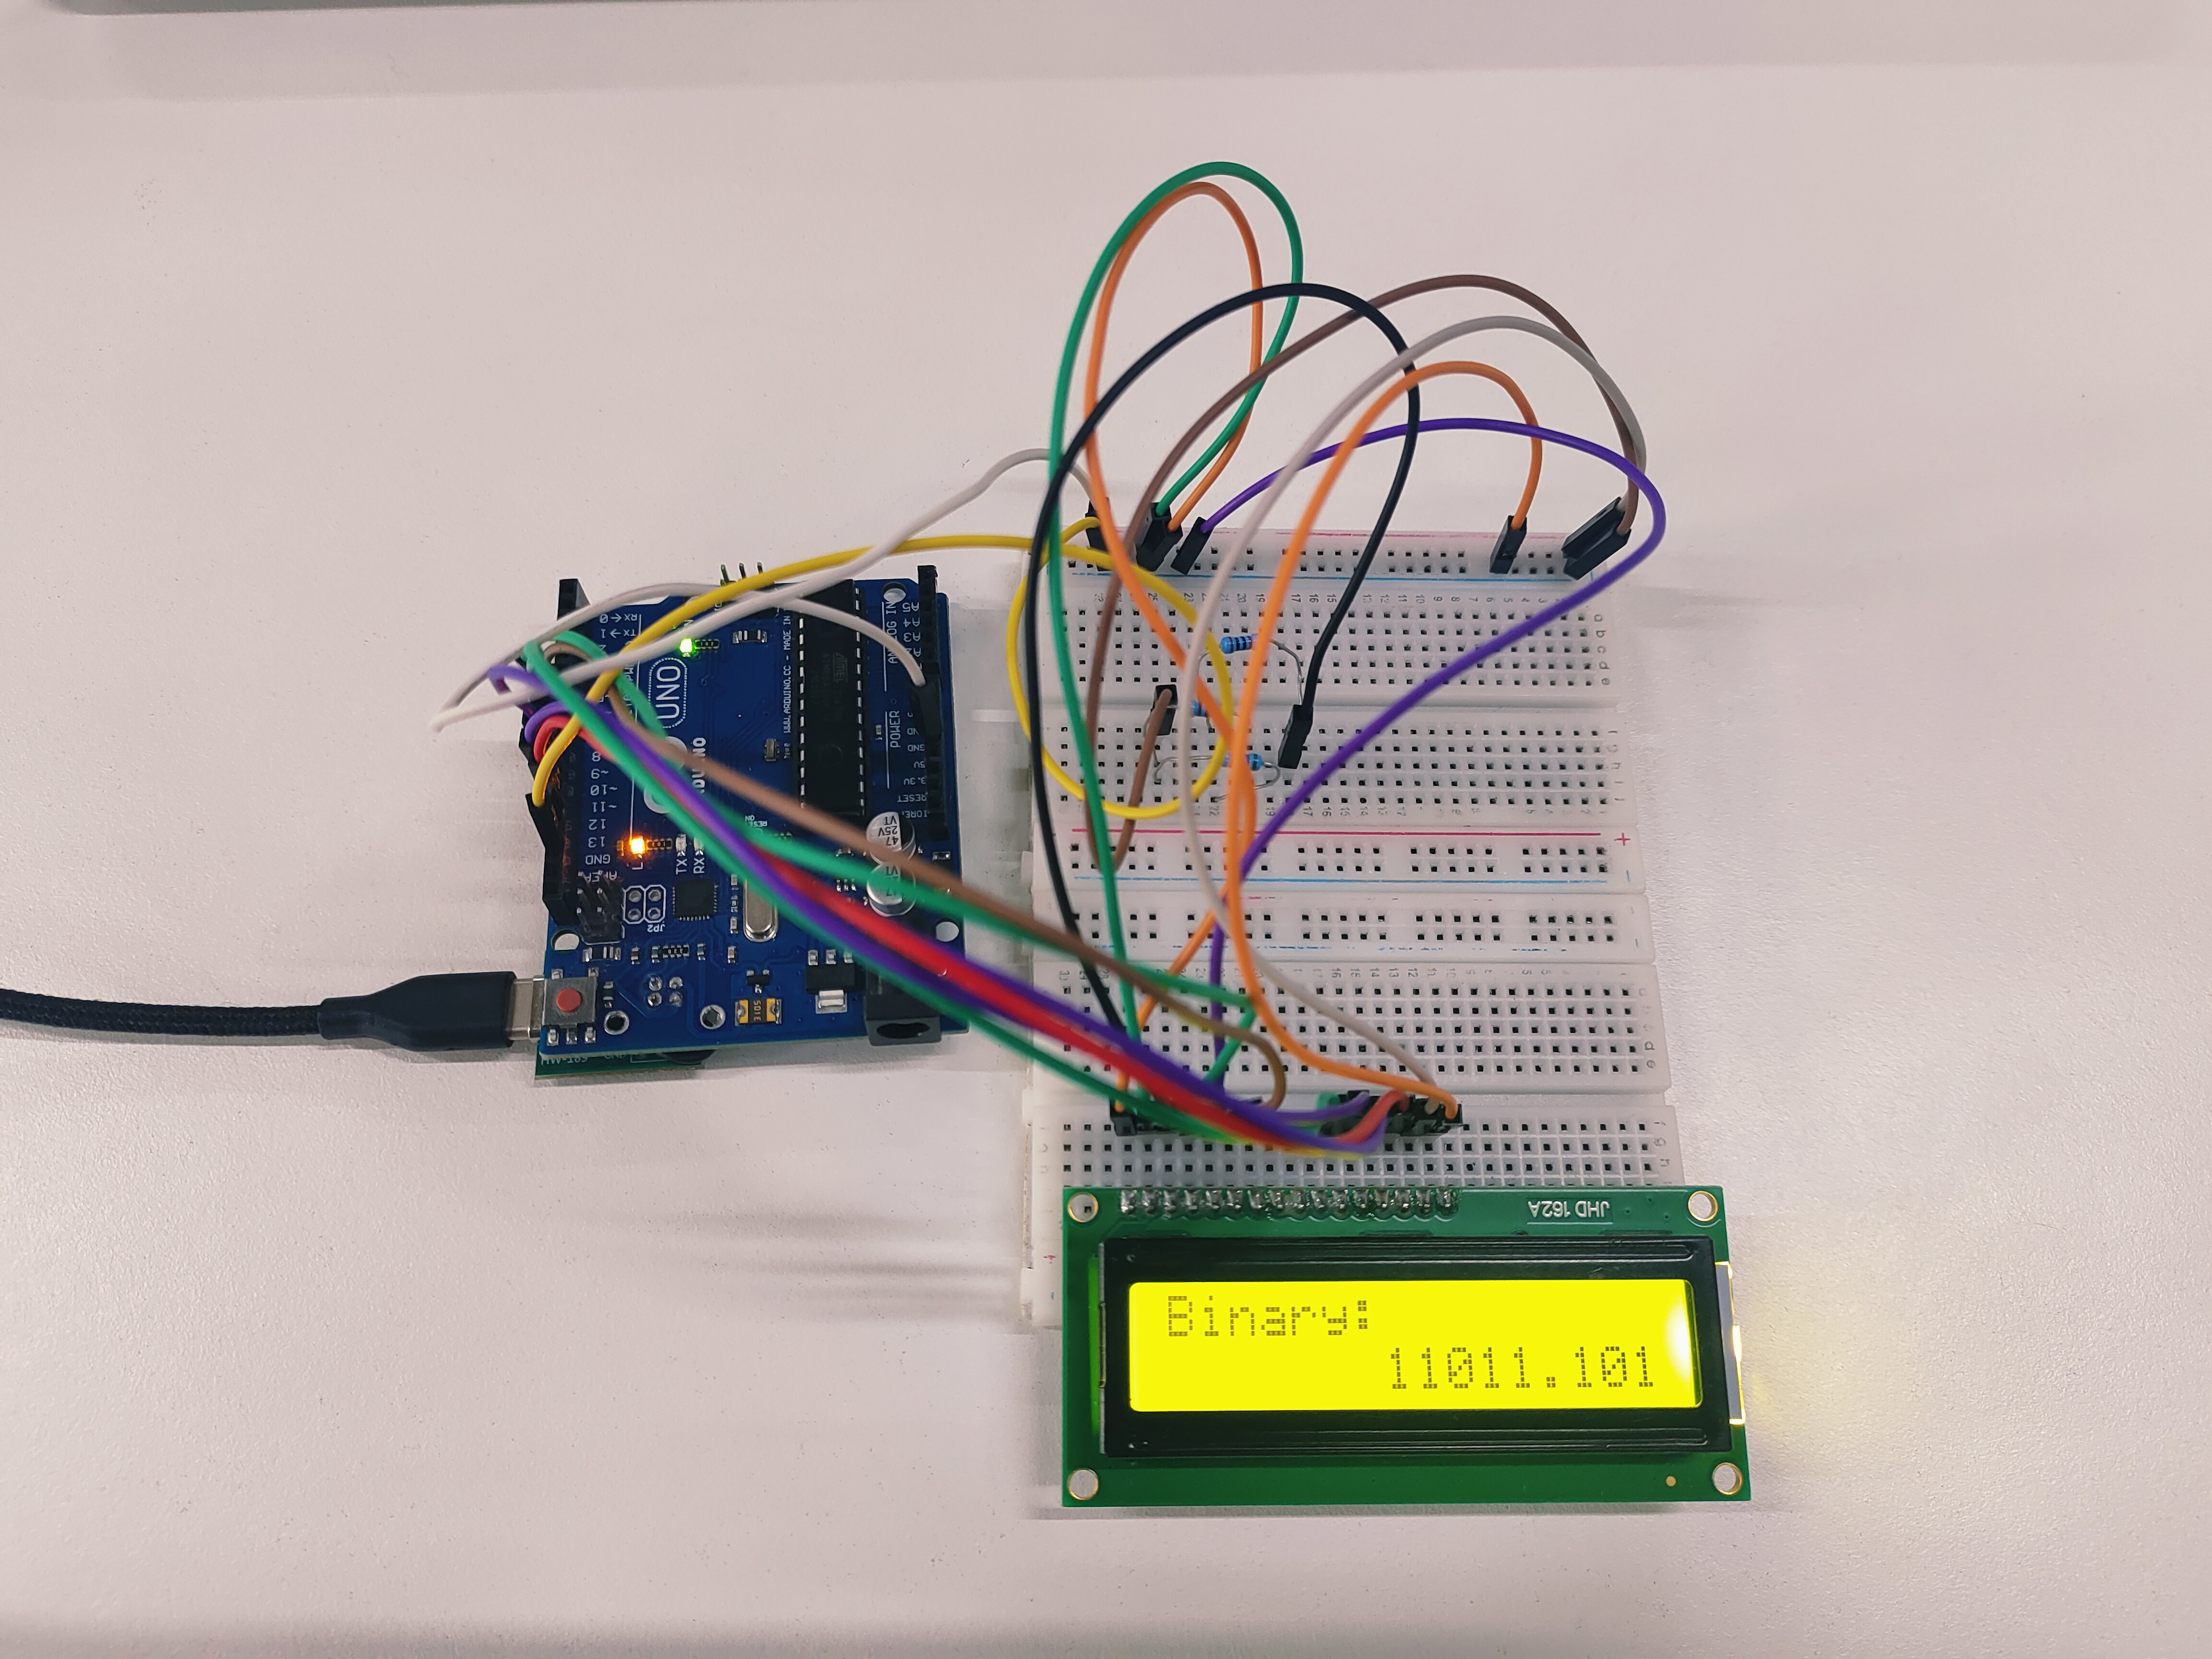
\includegraphics[width=\columnwidth]{figs/binary_out.jpg}
\caption{Binary value}
\label{fig:lcd}
\end{figure}
 \bibliographystyle{ieeetr}
\end{document}